% !TEX program = xelatex
%\documentclass[notes=onlyslideswithnotes,notes=hide]{beamer}
%\documentclass[notes=show]{beamer}
%\documentclass[handout]{beamer}
\documentclass[notes=hide]{beamer}
%\documentclass[notes=only]{beamer}
%\documentclass[10pt,letterpaper]{article}
%\usepackage{beamerarticle}

\usepackage{newtxtext}
\usepackage{genchem}
\usepackage{lecture}
\usepackage{ccicons}
\usepackage{bucolors}

\title{The Quantum-Mechanical Model of the Atom}
\subtitle{Chapter 2}
\institute[CHEM115 Bloomsburg University]{CHEM115 --- Chemistry for the Sciences I \\ Bloomsburg University}
\author{D.A.\ McCurry}
\date{Fall 2021}

\begin{document}

\maketitle
\mode<article>{\thispagestyle{fancy}}

\mode<presentation>{%
	{\usebackgroundtemplate{\includegraphics[width=\paperwidth]{solarpanels.png}}
	\begin{frame}[plain]
		\null
	\end{frame}
}}

\frame{\section{The Nature of Light}
	\begin{learningobjectives}
	\item Understand the particle and wave nature of light.
	\item Use equations to convert between energy, frequency, and wavelength.
	\item Be aware of tricky unit conversions.
	\end{learningobjectives}
}

\begin{frame}{Light is a Wave}
	\begin{center}
		\includegraphics[scale=0.4,trim={0 0 0 40pt},clip]{emrad.jpeg}
	\end{center}

	\begin{itemize}
		\item All electromagnetic waves move through space (in a vacuum)
			at the same, constant speed of
			\alert{\SI{3.00e8}{\meter\per\second}}.
	\end{itemize}
\end{frame}

\begin{frame}[allowframebreaks]{Properties of Waves}
	\note{%
	\begin{center}
		\includegraphics[scale=0.4]{wave-props.jpeg}
	\end{center}

	\begin{tabularx}{\linewidth} {>{\bfseries}r X}
		Wavelength ($\lambda$): & the distance between two peaks
			(maxima). \\
		Amplitude: & vertical height of the peak. \\
		Frequency ($\nu$): & the number of cycles (peaks) to pass
			through a stationary point in a given time period.
	\end{tabularx}
}

	\begin{center}
		\includegraphics[scale=0.4]{wave-props2.jpeg}
	\end{center}
\end{frame}

\begin{frame}[t]{Finding Relationships via Dimensional Analysis}
	We have\ldots

	\begin{center}
		\begin{tabular} {>{\ldots~}l  c s l}
			wavelength     & $\lambda$ & \nano\meter       & length \\
			frequency      & $\nu    $ & 1\per\second      & time \\
			speed of light & $c      $ & \meter\per\second & length and time \\
		\end{tabular}
	\end{center}

	\note{%
		\begin{equation*}
			c = \lambda v \qquad\text{\em or}\qquad \lambda = \frac{c}{\nu} \qquad\text{\em or}\qquad \nu = \frac{c}{\lambda}
		\end{equation*}
	}
\end{frame}

\begin{frame}{The Electromagnetic Spectrum}
	Different $\lambda$ of light correspond to different energy regions of
	the electromagnetic spectrum.
	\begin{center}
		\includegraphics[scale=0.45,trim={0 0 0
		30pt},clip]{emspectrum.jpeg}
	\end{center}
\end{frame}

\begin{frame}{A Qualitative Comparison of Waves}
	Consider these two waves:

	\bigskip

	\begin{columns}
		\column{0.5\linewidth}
	\begin{center}
		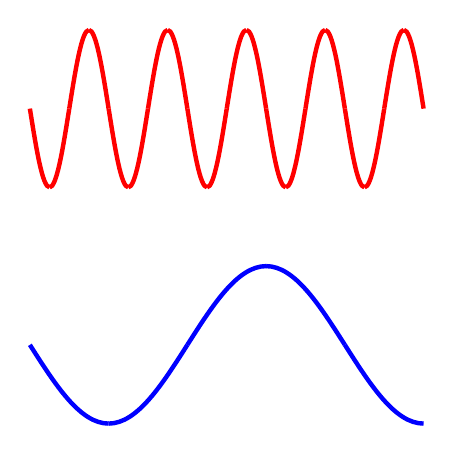
\begin{tikzpicture}
			\foreach \x in {0,1,...,4}{
				\draw[ultra thick, red] (\x,0) sin (\x+0.25,-1);
				\draw[ultra thick, red] (\x+0.25,-1) cos (\x+0.5,0);
				\draw[ultra thick, red] (\x+0.5,0) sin (\x+0.75,1);
				\draw[ultra thick, red] (\x+0.75,1) cos (\x+1,0);
				};
			\draw[ultra thick, blue] (0,-3) sin (1,-4);
			\draw[ultra thick, blue] (1,-4) cos (2,-3);
			\draw[ultra thick, blue] (2,-3) sin (3,-2);
			\draw[ultra thick, blue] (3,-2) cos (4,-3);
			\draw[ultra thick, blue] (4,-3) sin (5,-4);
		\end{tikzpicture}
	\end{center}
		\column{0.4\linewidth}

	\begin{enumerate}[<+(1)->]
		\item Which has the higher frequency?
		\item If one of these represents visible light and the other IR
			radiation, which is which?
	\end{enumerate}
	\end{columns}
\end{frame}

\begin{frame}[t]{Frequency to Wavelength}
	A photon has a frequency of \SI{6.0e14}{\hertz}. Convert this frequency
	into wavelength (\si{\nano\meter}). Does this frequency fall in the
	visible region? ($c = \SI{3.0e8}{\meter\per\second}$)

	\note{
		\begin{tabularx}{\linewidth} {@{}*{3}{>{\centering\arraybackslash}X}}
			\toprule\bfseries Given & \bfseries Plan & \bfseries Find \\ \midrule
			\SI{6.0e14}{\hertz}      & $c = \SI{3.00e8}{\meter\per\second}$ & \si{\nano\meter} \\
			\SI{6.0e14}{\per\second} & $\SI{1e9}{\nano\meter} = \SI{1}{\meter}$ \\
			\bottomrule
		\end{tabularx}

		\begin{align*}
			\frac{\num{6.0e14}}{\si{\second}} \times \frac{\si{\second}}{\SI{3.00e8}{\meter}} \times \frac{\SI{1}{\meter}}{\SI{1e9}{\nano\meter}} &= \SI{0.002}{\per\nano\meter} \\
			(\SI{0.002}{\per\nano\meter})^{-1} &= \SI{500}{\nano\meter} \\
			&= \boxed{\SI{5.0e2}{\nano\meter}}
		\end{align*}

		\fbox{Yes.}
		}
\end{frame}

\begin{onyourown}%{15em}
	A photon has a frequency of \SI{3.4e12}{\hertz}. Convert this frequency
	into wavelength (\si{\nano\meter}). Does this frequency fall in the
	visible region?
\end{onyourown}

\clearpage

\begin{frame}{The Wave Nature of Light}{Interference}
	\centering

	\includegraphics[scale=0.4]{constructive-interference.jpeg}

	\bigskip

	\includegraphics[scale=0.4]{destructive-interference.jpeg}
\end{frame}

\begin{frame}[allowframebreaks]{The Wave Nature of Light}{Diffraction}
	\begin{center}
		\includegraphics[scale=0.38]{diffraction.jpeg}
	\end{center}

	\framebreak%

	\begin{center}
		\includegraphics[scale=0.38]{diffraction-interference.jpeg}
	\end{center}
\end{frame}

\begin{frame}{The Particle Nature of Light}{The Photoelectric Effect}
	\begin{center}
		\includegraphics[scale=0.4,trim={0 20pt 0 40pt},clip]{photoelectric-effect.jpeg}
	\end{center}

	\begin{description}[<+->]
		\item[Theory:] Energy from light would need to exceed binding
			energy of electron.
			\note{%
			\begin{itemize}
				\item Short $\lambda$, high energy light
				\item Long $\lambda$, low energy light over
					extended time
			\end{itemize}}
		\item[Observation:] No matter how long the low energy light was
			used, electrons were not emitted.
	\end{description}
\end{frame}

\begin{frame}{The Quantum Nature of Light}
	\begin{block}{The Particle-Wave Duality}
		Light can act as both a particle and a wave.
	\end{block}

	\begin{itemize}
		\item Light is composed of photons -- ``packets'' of a specific
			energy (\alert{quantized})
		\item Depend only on frequency, $E = h \nu$
			\begin{itemize}
				\item inversely proportional to $\lambda$
				\item proportionality constant -- \alert{Planck's
					Constant ($h$)}

					\begin{equation*}
						h =
						\SI{6.626e-34}{\joule\second}
					\end{equation*}
			\end{itemize}
	\end{itemize}
\end{frame}

\note{%
A little rearrangement\ldots
	\begin{align*}
		\intertext{From before:}
		\nu &= \frac{c}{\lambda}
		\intertext{We now have:}
		E &= h\nu
		\intertext{Therefore,}
		E &= \frac{hc}{\lambda}
	\end{align*}
}

\begin{frame}[t]{Wavelength to Energy}
	When copper is bombarded with high-energy electrons, X-rays are emitted.
	Calculate the energy (in \si{\joule}) associated with the photons if the
	wavelength of the X-rays is \SI{0.154}{\nano\meter}. ($h =
	\SI{6.63e-34}{\joule\second}$)

	\note{%
		\begin{tabularx}{\linewidth} {@{}*{3}{>{\centering\arraybackslash}X}}
			\toprule\bfseries Given & \bfseries Plan & \bfseries Find \\ \midrule
			$\lambda = \SI{0.154}{\nano\meter}$ & $E = \frac{hc}{\lambda}$ & \si{\joule} \\
			\bottomrule
		\end{tabularx}

		\begin{align*}
			E &= \frac{hc}{\lambda} \\
			&= \frac{(\SI{6.63e-34}{\joule\second})(\SI{3.00e8}{\meter\per\second})}{\SI{0.154}{\nano\meter}} \times \frac{\SI{1e9}{\nano\meter}}{\SI{1}{\meter}} \\ &= \SI{1.29156e-15}{\joule} \\
			&= \boxed{\SI{1.29e-15}{\joule}}
		\end{align*}
			}
\end{frame}

%\begin{onyourown}%{10em}
%	All metals, in fact, emit X-rays when bombarded with high-energy
%	electrons. Calculate the energy (in \si{\joule}) associated with the photons if
%	the wavelength of the X-rays is \SI{0.107}{\nano\meter}.
%\end{onyourown}

\begin{frame}[t]{Energy in a Mole}
	Calculate the energy of a photon with a
	frequency of \SI{5.09e13}{\per\second}. How much energy would
	\SI{1}{\mole} of these photons contain?

	\note{\footnotesize
		\begin{tabularx}{\linewidth} {@{}*{3}{>{\centering\arraybackslash}X}}
			\toprule\bfseries Given & \bfseries Plan & \bfseries Find \\ \midrule
			$\nu = \SI{5.09e13}{\per\second}$ & $E = h \nu$  & \si{\joule\per\mole} \\
			& $\SI{1}{\mole} = \num{6.022e23}$ \\
			& $h = \SI{6.63e-34}{\joule\second}$ \\
			\bottomrule
		\end{tabularx}

		\begin{align*}
			E_{\SI{1}{photon}} &= h\nu
			= (\SI{6.63e-34}{\joule\second})(\SI{5.09e13}{\per\second}) \\
			&= \SI{3.37467e-20}{\joule} \\
			E_{\SI{1}{\mole}} &= \SI{3.37467e-20}{\joule\per photon} \times \frac{\SI{6.022e23}{photons}}{\SI{1}{\mole}} \\
			&= \SI{20315.5134}{\joule\per\mole}
			= \boxed{\SI{20.3e3}{\joule\per\mole}} \\
			\intertext{Often expressed as\ldots}
			&= \boxed{\SI{20.3}{\kilo\joule\per\mole}}
		\end{align*}}
\end{frame}

\begin{onyourown}%{14em}
	Calculate the energy of a photon with a frequency of
	\SI{3.42e15}{\per\second}. How much energy would \SI{0.5}{\mole} of
	these photons contain?
\end{onyourown}

\frame{\section{The Quantum Nature of the Atom}
	\begin{learningobjectives}
	\item Explain the similarities between electrons and photons.
	\item Use the de Broglie equation to calculate the wavelength of particles.
	\end{learningobjectives}
}

\begin{frame}[allowframebreaks]{Emission Spectra}
	\begin{center}
		\includegraphics[scale=0.3,trim={0 30pt 0 0},clip]{lamp-emission.jpeg}
	
		\includegraphics[scale=0.3,trim={0 30pt 0 0},clip]{emission-spectra.jpeg}
	\end{center}

	\framebreak

	\begin{center}
		\includegraphics[scale=0.35]{emission-spectra2.jpg}
	\end{center}
\end{frame}

\note{%
Bohr's Model of the Atom (1913)
	\begin{itemize}
		\item Electrons could only have \alert{very specific amounts} of
			energy.
		\item Electrons traveled in orbitals that were a fixed distance
			from the nucleus.
			\begin{itemize}
				\item \alert{Stationary states}
				\item The energy of the electron was
					proportional to the distance the orbital
					was from the nucleus.
			\end{itemize}
		\item Electrons emitted radiation when they ``jumped'' from an
			orbit with higher energy down to an orbit with lower
			energy.
			\begin{itemize}
				\item The distance between the orbitals determined
					the energy of the photon of light
					produced.
			\end{itemize}
	\end{itemize}
}

%\begin{frame}{Orbitals?}
%	\centering
%
%	\includegraphics[scale=0.8]{stylized-li-atom.pdf}
%
%	\bigskip
%
%	\tiny\ccbysa\ Indolences
%\end{frame}

\note{%
 The Bohr Model and Emission Spectra
 \begin{center}
	\includegraphics[scale=0.35,trim={0 0 0 40pt},clip]{bohr-model.jpeg}
\end{center}
}

\note{%
Electron Transitions
	\begin{columns}
		\column{0.5\linewidth}
		\begin{itemize}
			\item Electrons can exist \alert{only} in certain
			     orbitals (not in between).
			\item Light \alert{emission} is a result of an
			     \alert{electron transition} from a higher energy
			     orbital to one of lower energy.
			\item Light \alert{absorption} is a result of an
				\alert{electron transition} from a lower energy
				orbital to one of higher energy.
		\end{itemize}
		\column{0.5\linewidth}
		\begin{center}
		\begin{tikzpicture}[hv/.style={->,decorate,decoration={snake,
			amplitude=2pt,segment length=10pt,post=lineto,post
			length=2pt},red}]
			\draw[very thick,->] (0,-5) -- (0,0) node[midway,left] {$E$};
			\draw[thick] (0.2,-1) -- (1.2,-1) node[at end,right]
			{\alert{Excited State}};
			\draw[thick] (0.2,-4) -- (1.2,-4) node[at end,right]
			{\alert{Ground State}};
			\only<1>{\draw[thick,<->,inner sep=10pt] (0.7,-1.1) --
			(0.7,-3.9) node[midway,right] {$\Delta E$};}
			\only<2|handout:0|article:0>{\draw[thick,->] (0.7,-1.1) -- (0.7,-3.9);
			\draw[hv] (0.8,-2.5) -- (2.3,-2.5) node[midway,above]
			{$h\nu$} node[at end,right] {$\Delta E < 0$};}
			\only<3|handout:0|article:0>{\draw[thick,<-] (0.7,-1.1) -- (0.7,-3.9);
			\draw[hv] (2.3,-2.5) -- (0.8,-2.5) node[midway,above]
			{$h\nu$} node[at start,right] {$\Delta E > 0$};}
		\end{tikzpicture}
		\end{center}
	\end{columns}
}

\begin{frame}{Hydrogen Energy Transitions and Radiation}
	\centering
	\includegraphics[scale=0.45,trim={0 0 0 30pt},clip]{H-transitions.jpeg}
\end{frame}

\begin{frame}{Calculating Energy Differences}
	Consider the following energy levels of a hypothetical atom:

	\begin{columns}
		\column{0.45\linewidth}
		\begin{center}
			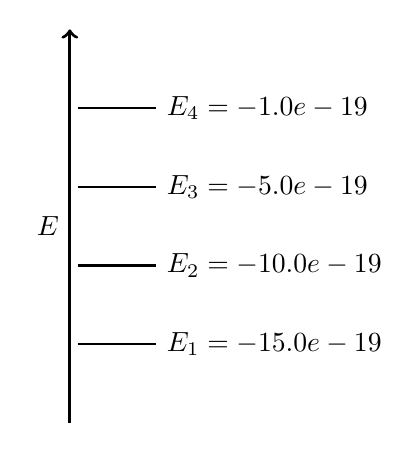
\begin{tikzpicture}
				\draw[very thick,->] (0,-1) -- (0,4) node[midway,left] {$E$};
				\draw[thick] (0.1,3) -- ++(1,0) node[at end,right]{$E_4 = \SI{-1.0e-19}{\joule} $};
				\draw[thick] (0.1,2) -- ++(1,0) node[at end,right]{$E_3 = \SI{-5.0e-19}{\joule} $};
				\draw[thick] (0.1,1) -- ++(1,0) node[at end,right]{$E_2 = \SI{-10.0e-19}{\joule}$};
				\draw[thick] (0.1,0) -- ++(1,0) node[at end,right]{$E_1 = \SI{-15.0e-19}{\joule}$};
			\end{tikzpicture}
		\end{center}
		\column{0.45\linewidth}
		\begin{enumerate}
			\item What is the energy (in \si{\joule}) a photon must
				have in order to excite an electron from $E_2$
				to $E_3$?
				\note[item]{
					\begin{tabular} {c
						S[table-format=-2.1e-2]<{
							\si{\joule}}}
							& -5.0e-19 \\
							$-$ &-10.0e-19 \\
							\midrule
							& 5.0e-19
					\end{tabular}}
			\item What is the wavelength of the photon emitted when
				an electron goes from $E_4$ to $E_1$?
				\note[item]{
					\begin{tabular} {c
						S[table-format=-2.1e-2]<{
							\si{\joule}}}
							& -15.0e-19 \\
							$-$ &-1.0e-19 \\
							\midrule
							& -14.0e-19
					\end{tabular}}
		\end{enumerate}
	\end{columns}
\end{frame}

\begin{onyourown}%{0em}
	\begin{enumerate}
		\item What is the energy (in \si{\joule}) a photon must
			have in order to excite an electron from $E_1$
			to $E_3$?
		\item What is the wavelength of the photon \alert{absorbed} when
			an electron goes from $E_1$ to $E_4$?
	\end{enumerate}
\end{onyourown}

\begin{frame}{Wave Behavior of Electrons}
	\note{%
		\begin{itemize} 
			\item Louis de Broglie (1924) -- Particles of \alert{all} sizes
				have both particle and wave properties.
			\item The wave character is only significant for sub-atomic
				particles (very small mass).
			\item Electron beams show an interference pattern!
				\begin{itemize}
					\item The electrons interfere with
						themselves.
				\end{itemize}
%			\item<2-> How do we calculate the frequency or
%				wavelength of an electron?
		\end{itemize}
	}
	\begin{center}
		\includegraphics[scale=0.5]{electron-interference-edit.jpeg}
	\end{center}
\end{frame}

\begin{frame}{The de Broglie Wavelength}
	de Broglie predicted that the wavelength of a particle was
	\alert{inversely proportional} to its \alert{momentum}:

	\begin{align*}
		\text{Momentum} &= mv \\
		\intertext{where $m$ is mass and $v$ is velocity.}
		\lambda &= \frac{h}{mv} \\
	\end{align*}

	\begin{center}
		\bfseries\usebeamercolor[fg]{alerted text} If we know the velocity of an electron, we also know its
		wavelength.
	\end{center}
\end{frame}

\begin{frame}[t]{Calculating the de Broglie Wavelength}
	\onslide<+->
	What is the de Broglie wavelength (in \si{\nano\meter}) associated with
	a \SI{143}{\gram} baseball traveling at \SI{40.0}{\meter\per\second}?

	\vspace{\stretch{1}}

	\note{\footnotesize
		\begin{tabularx}{\linewidth} {@{}*{3}{>{\centering\arraybackslash}X}}
			\toprule\bfseries Given & \bfseries Plan & \bfseries Find \\
			\midrule
			$m = \SI{143}{\gram}$ & $\lambda = \frac{h}{mv}$ &
			\si{\nano\meter} \\
			$v = \SI{40.0}{\meter\per\second}$ & $h =
			\SI{6.626e-34}{\joule\second}$ \\ \bottomrule
		\end{tabularx}

		\begin{align*}
			\lambda &= \frac{h}{mv}
			=
			\frac{\SI{6.626e-34}{\joule\second}}{(\SI{143}{\gram})(\SI{40.0}{\meter\per\second})}
			\\
			\intertext{Seconds cancels out\ldots but what about
			joules?}
			&= \frac{\SI{6.626e-34}{\joule\second}}{(\SI{143}{\gram})(\SI{40.0}{\meter\per\second})}
			\times
			\frac{\SI{1}{\kilo\gram\meter\squared\per\second\squared}}{\SI{1}{\joule}}
			\times \frac{\SI{1000}{\gram}}{\SI{1}{\kilo\gram}}
			\times \frac{\SI{e9}{\nano\meter}}{\SI{1}{\meter}} \\
			&= \SI{1.15839e-25}{\nano\meter} =
			\boxed{\SI{1.16e-25}{\nano\meter}}
		\end{align*}

		Way too small to ever measure.}


	\onslide<+->
	What is the de Broglie wavelength (in \si{\nano\meter}) associated with
	an electron traveling at \SI{62}{\meter\per\second}?

	$(\text{mass of an electron} = \SI{9.1e-31}{\kilo\gram})$

	\vspace{\stretch{1}}

\end{frame}

\note{%
		\begin{tabularx}{\linewidth} {@{}*{3}{>{\centering\arraybackslash}X}}
			\toprule\bfseries Given & \bfseries Plan & \bfseries Find \\
			\midrule
			$m = \SI{9.1e-31}{\kilo\gram}$ & $\lambda = \frac{h}{mv}$ &
			\si{\nano\meter} \\
			$v = \SI{62}{\meter\per\second}$ & $h =
			\SI{6.626e-34}{\joule\second}$ \\ \bottomrule
		\end{tabularx}

		\begin{align*}
			\lambda &= \frac{h}{mv} \\
			&=
			\frac{\SI{6.626e-34}{\joule\second}}{(\SI{9.1e-31}{\kilo\gram})(\SI{62}{\meter\per\second})}
			\times
			\frac{\SI{1}{\kilo\gram\meter\squared\per\second\squared}}{\SI{1}{\joule}}
			\times \frac{\SI{e9}{\nano\meter}}{\SI{1}{\meter}} \\
			&= \SI{11744}{\nano\meter} = \boxed{\SI{1.2e4}{\nano\meter}}
		\end{align*}

		Infrared region
		}

%\begin{onyourown}%{10em}
%	If a \SI{1650}{\kilo\gram} car has a de Broglie wavelength of
%	\SI{3.82e-33}{\nano\meter}, how fast was the car moving in
%	\si{\kilo\meter\per\second}?
%\end{onyourown}


\begin{frame}{Testing the Wave Behavior of Electrons}
	\begin{center}
		\includegraphics[scale=0.4]{testing-e-wave.jpeg}
	
		\pause
	
		\bfseries\usebeamercolor[fg]{alerted text} The more we know about the wave-like behavior, the less we
		know about the particle-like behavior.
	\end{center}
\end{frame}

\clearpage

\frame{\section{Uncertainty}
	\begin{learningobjectives}
	\item Understand that it is impossible to know the exact position of an electron.
	\item Be familiar with the idea of probability distributions.
	\item Identify every unique electron in an atom using quantum numbers.
	\end{learningobjectives}
}

\begin{frame}{Uncertainty}
	The wave nature and particle nature of electrons are
	\alert{complementary properties}.
	\begin{itemize}
		\item They both describe the electron, but\ldots
		\item Neither has any effect on the other property.
	\end{itemize}

	\begin{block}{Heisenberg's Uncertainty Principle}
		\begin{equation*}
			\Delta x \times m \Delta v \geq \frac{h}{4\pi}
		\end{equation*}

		The more we know about the position of an electron, the less we
		know about its velocity.
	\end{block}
\end{frame}

\begin{frame}{Schrödinger's Cat}
	\centering
	\includegraphics[scale=0.2]{Schrodingers-cat.pdf}

	\footnotesize \ccbysa\ Dhatfield
\end{frame}


%\mode<presentation>{
%\begin{frame}
%	\begin{columns}
%		\column{0.45\linewidth}
%		\begin{itemize}
%			\item Is he a good husband/father?
%			\item Is he a meth expert?
%			\item<2-> \alert{Can he be both?}
%		\end{itemize}
%		\column{0.45\linewidth}
%		\includegraphics[width=\linewidth]{WalterWhite.jpg}
%	\end{columns}
%\end{frame}}

\begin{frame}[allowframebreaks=1]{Indeterminacy}
		Newton's law of motion are deterministic
			\begin{itemize}
				\item Present determines future.
				\item All things equal, you should get the same
					result every time.
				\item We know velocity and position.
			\end{itemize}
			\begin{center}
				\includegraphics[scale=0.4]{trajectory.jpeg}
			\end{center}

			\framebreak

		Electrons do not work this way
		\begin{itemize}
			\item All things equal, you will \alert{never}
				get the same result.
			\item A game of statistics.
		\end{itemize}

		\begin{center}
			\includegraphics[scale=0.4]{indeterminacy.jpeg}
		\end{center}

		\begin{center}
			\bfseries\usebeamercolor[fg]{alerted text} There is a likely place where electrons will be,
			but we don't know the exact position.
		\end{center}
\end{frame}

\begin{frame}[t]{Probability and the Atom}
	\begin{block}{The Schrödinger Equation}
		Describes both the particle and wave nature of an electron:
		\begin{equation*}
			H\Psi = E\Psi
		\end{equation*}
		The wave function ($\Psi$) describes
		\begin{enumerate}
			\item The energy of an electron.
			\item The probability of finding an electron in a volume
				of space.
		\end{enumerate}
	\end{block}

	\mode<presentation>{
	\only<2-3>{The math gets complicated pretty quickly\ldots
	\begin{equation*}
		\alt<3>{\xcancel{ i\hbar \frac{\partial \Psi}{\partial t} =
		-\frac{\hbar^2}{2m} \frac{\partial^2 \Psi}{\partial x^2} + V
		\Psi}}{i\hbar \frac{\partial \Psi}{\partial t} =
		-\frac{\hbar^2}{2m} \frac{\partial^2 \Psi}{\partial x^2} + V
		\Psi}
	\end{equation*}
		\visible<3>{So we won't worry about it. Take CHEM361.}}}

%\only<4->{\begin{itemize}
%	\item This has only been solved exactly for the hydrogen atom.
%	\item Multi-electron systems require \alert{approximations}.
%	\end{itemize}}
\end{frame}

\begin{frame}{The Schrödinger Wave Equation}
	We can still use the equation for useful predictions:
	\begin{itemize}
		\item The probability distribution map showing where an electron is likely to be found is called an
			\alert{orbital}.
		\item Each orbital is specified by three interrelated quantum numbers and a fourth quantum number that
			specifies the spin of the electron.
			\begin{center}
				\begin{tabular} {>{$}c<{$}@{\qquad} l}
					n   & Principal quantum number        \\
					l   & Angular Momentum quantum number \\
					m_l & Magnetic quantum number         \\
					m_s & Spin quantum number             
				\end{tabular}
			\end{center}
	\end{itemize}
\end{frame}

\begin{frame}{Principal Quantum Number}
	\begin{itemize}
		\item Determines the overall \alert{size} and \alert{energy} of an orbital.
		\item Orbitals with the same value of $n$ are in the \alert{same}
			principal level/shell.
	\end{itemize}

	\begin{equation*}
		n = 1, 2, 3, 4, \ldots
	\end{equation*}

	\begin{columns}
		\column{0.45\linewidth}
		\begin{center}
		\includegraphics[scale=0.2]{rhydberg-h.jpeg}
		\end{center}
		\column{0.45\linewidth}
		\begin{align*}
			R_{\ch{H}} &= \SI{2.18e-18}{\joule} \\
			E_n &= -R_{\ch{H}}\bigg(\frac{Z^2}{n^2}\bigg)
			=
			\underbrace{-R_{\ch{H}}\bigg(\frac{1}{n^2}\bigg)}_{\mathclap{\text{for
			hydrogen}}}
		\end{align*}

		\pause

		How does the distance between shells change as $n$ continues to
		get larger?
	\end{columns}
\end{frame}

\begin{frame}{Angular Momentum Quantum Number}
	\begin{itemize}
		\item Determines the \alert{shape} of an orbital.
		\item Electrons all have the same relative energy within each
			\alert{sublevel}.
	\end{itemize}
	\begin{equation*}
		l = 0, 1, 2, 3, 4, 5, \ldots =
		s, p, d, f, g, h, \ldots
	\end{equation*}

	Valid values for $l$ range from 0 to $n-1$, so
	\begin{center}
		\begin{tabular} {l l l}
			\toprule\bfseries $\bm{n}$ &
			\multicolumn{2}{l}{\bfseries Possible values
			of $\bm{l}$} \\
		\midrule
			1 & 0          & $s$ \\
			2 & 0, 1       & $s$, $p$ \\
			3 & 0, 1, 2    & $s$, $p$, $d$ \\
			4 & 0, 1, 2, 3 & $s$, $p$, $d$, $f$ \\
			\ldots & \ldots & \ldots \\ \bottomrule
	\end{tabular}
	\end{center}
\end{frame}

\begin{frame}{Shape of an Orbital?}
	\centering
	\includegraphics[scale=0.2,trim={0 700pt 0 0},clip]{orbitalshape.jpg}

	\footnotesize \url{https://chem.libretexts.org}
\end{frame}

\begin{frame}{Magnetic Quantum Number}
	\begin{itemize}
		\item Determines the \alert{orientation} of an orbital.
	\end{itemize}
	\begin{equation*}
		m_l = \ldots, -3, -2, -1, 0, +1, +2, +3, \ldots
	\end{equation*}

	Valid values for $m_l$ range from $\pm l$, so

	\begin{center}
		\begin{tabularx}{2.5in} {c c >{\raggedleft\arraybackslash}X@{~0,~}X}
			\toprule\bfseries $\bm{n}$ & $\bm{l}$ &
			\multicolumn{2}{c}{\bfseries Possible values
			of $\bm{m_l}$} \\
		\midrule
			1 & 0 &          &    \\
			2 & 0 &          &    \\
			  & 1 & -1,      & +1 \\
			3 & 0 &          &    \\
			  & 1 & -1,      & +1 \\
			  & 2 & -2, -1,  & +1, +2 \\
			\ldots & \ldots & \multicolumn{2}{c}{\ldots} \\ \bottomrule
	\end{tabularx}
	\end{center}
\end{frame}

\begin{frame}{Spin Quantum Number}
	\begin{itemize}
		\item Associated with the electron, not the orbital.
		\item Describes the \alert{spin} of an electron.
		\item All electrons have the same \alert{magnitude} of spin, just
			a different \alert{direction}.
	\end{itemize}
	\begin{equation*}
		m_s = +\frac{1}{2}, -\frac{1}{2}
	\end{equation*}

	\begin{center}
		\includegraphics[scale=0.25]{spin-mcmurry.jpg}
	\end{center}
\end{frame}

\begin{frame}{General Trends in Quantum Numbers}
	\begin{columns}
		\column{0.4\linewidth}
	\begin{itemize}
		\item Number of sublevels in any level is equal to $n$.
		\item Number of orbitals in a sublevel is $2l + 1$.
		\item Total number of orbitals in a level is $n^2$.
	\end{itemize}
		\column{0.6\linewidth}
	\begin{center}
		\includegraphics[scale=0.35]{sublevels.jpeg}
	\end{center}
	\end{columns}
\end{frame}

\begin{frame}{Probability and Radial Distribution Functions}
	How do we get the \alert{shapes} of atomic orbitals?
	\begin{itemize}
		\item $\Psi^2$ is the \alert{probability density}.
			\begin{itemize}
				\item The probability of finding an electron at
					a particular point in space.
				\item Electrons are \alert{forbidden} and have a
					\alert{0\% probability} of being found at
					\alert{nodes}.
			\end{itemize}
	\end{itemize}

	\bigskip

	\begin{columns}
		\column{0.45\linewidth}
		Assume $\Psi$ is a sine wave:

		\begin{center}
			\begin{tikzpicture}[scale=0.6]
				\tikzstyle{nodelabel}=[blue,draw,thick];
				\tikzstyle{nodearrow}=[->,shorten >=3pt,thick,blue];
			\begin{axis}[axis x line=middle,
				axis y line=left,
				tick label style={font=\Large},
				xmin=0,
				xmax=8.5,
				ymin=-1.5,
				ymax=1.5,
				ytick={-1,0,1},
				y axis line style={<->},
				xtick=\empty,
				domain=-0.1:8.5,]
				\addplot[color=bumaroon,samples=200,ultra thick] {sin(x*90)};
				\only<2->{
					\node[style=nodelabel](A) at (axis cs:3,0.5) {Nodes};
				\draw[style=nodearrow] (A.south) to [in=30,out=270](axis
				cs:2,0);
				\draw[style=nodearrow] (A.south) to [in=150,out=270](axis
				cs:4,0);
				\node[style=nodelabel](B) at (axis cs:7,0.5) {Nodes};
				\draw[style=nodearrow] (B.south) to [in=30,out=270](axis
				cs:6,0);
				\draw[style=nodearrow] (B.south) to [in=150,out=270](axis
				cs:8,0);
				\node[style=nodelabel](C) at (axis cs:1,-0.5) {Node};
				\draw[style=nodearrow] (C.north) to
				[in=-30,out=90](axis cs:0,0);}
			\end{axis}
		\end{tikzpicture}
		\end{center}
		\column{0.45\linewidth}
		\visible<3->{
		If we square $\Psi$, we get $\Psi^2$:

		\begin{center}
			\begin{tikzpicture}[scale=0.6]
				\tikzstyle{nodelabel}=[blue,draw,thick];
				\tikzstyle{nodearrow}=[->,shorten >=3pt,thick,blue];
			\begin{axis}[axis x line=middle,
				axis y line=left,
				tick label style={font=\Large},
				xmin=0,
				xmax=8.5,
				ymin=-1.5,
				ymax=1.5,
				ytick={-1,0,1},
				y axis line style={<->},
				xtick=\empty,
				domain=-0.1:8.5,]
				\addplot[color=bumaroon,samples=200,ultra thick]
				{(sin(x*90))^2};
				\only<4->{
					\node[style=nodelabel](zero) at (axis cs:4.25,-0.75) {0\% Probability};
					\draw[style=nodearrow] (zero.north) to [in=-30,out=150](axis cs:0,0);
					\draw[style=nodearrow] (zero.north) to [in=-60,out=120](axis cs:2,0);
					\draw[style=nodearrow] (zero.north) to [in=-90,out=90](axis cs:4,0);
					\draw[style=nodearrow] (zero.north) to [in=240,out=60](axis cs:6,0);
					\draw[style=nodearrow] (zero.north) to [in=220,out=30](axis cs:8,0);
					\node[style=nodelabel,anchor=south,above,yshift=0.7em](high) at (current bounding box.north) {High Probability};
					\draw[style=nodearrow] (high.south) to [in=30,out=-150](axis cs:1,1);
					\draw[style=nodearrow] (high.south) to [in=0,out=-120](axis cs:3,1);
					\draw[style=nodearrow] (high.south) to [in=180,out=-80](axis cs:5,1);
					\draw[style=nodearrow] (high.south) to [in=140,out=-20](axis cs:7,1);
					}
			\end{axis}
		\end{tikzpicture}
		\end{center}}
	\end{columns}
\end{frame}

\begin{frame}{Translating Probability to 3D Orbitals}
	\centering
	\begin{columns}
		\column{0.3\linewidth}
		\begin{overlayarea}{\linewidth}{14em}
		\alt<2|handout:0>{\includegraphics[scale=0.27]{1sradialdist.jpeg}}
			{\includegraphics[scale=0.27,trim={0 40pt 360pt 0},clip]{1sprobability.jpeg}}
		\end{overlayarea}
			\column{0.3\linewidth}
			\includegraphics[scale=0.27,trim={0 30pt 330pt 0},clip]{1sdotdensity.jpeg}
			\column{0.3\linewidth}
		\includegraphics[scale=0.25]{1s3dshape.jpeg}
	\end{columns}
\end{frame}

\begin{frame}{Introducing Nodes to 3D Orbitals}
	\begin{columns}
		\column{0.4\linewidth}
		Whereas the $1s$ orbital did not have any nodes (the probability
		just trailed off), the $2s$, $3s$, etc. have \alert{at least} one
		node.

		\visible<2->{
			\begin{equation*}
				\parbox{\widthof{nodes}}{\centering \# of \alert{radial} nodes} = n - l - 1
			\end{equation*}}

		\column{0.6\linewidth}
		\centering
		\includegraphics[scale=0.4]{2s3snodes.jpeg}
	\end{columns}
\end{frame}

\begin{frame}{What about the other quantum numbers?}
	\begin{center}
		\begin{tikzpicture}
			\node(fig)
			{\includegraphics[width=\linewidth]{p-orbitals.jpeg}};
			\node[right,anchor=north west,align=left] at (fig.west)
			{\begin{minipage}{0.6\linewidth}
				\begin{itemize}
				\item $l$ describes the overall \alert{shape}.
					\begin{center}
						$s$, $p$, $d$, \ldots
					\end{center}
					\begin{equation*}
						l = \text{\# of \alert{angular}
						nodes}
					\end{equation*}
				\item $m_l$ describes the \alert{direction} the
					orbital is pointing.
					\begin{center}
						$p_{\bm{x}}$, $p_{\bm{y}}$,
						$p_{\bm{z}}$
					\end{center}
			\end{itemize}
			\end{minipage}};
		\end{tikzpicture}
	\end{center}
\end{frame}

\begin{frame}{The $d$ Orbitals\ldots}
	\centering
	\includegraphics[scale=0.45]{d-orbitals.jpeg}
	\begin{equation*}
		\text{Total \# Nodes (N)} = \underbrace{n - l -
		1}_{\mathclap{\text{\# radial}}} +
		\underbrace{l}_{\mathclap{\text{\# angular}}} = n - 1
	\end{equation*}
\end{frame}

\begin{frame}{The $f$ Orbitals\ldots}
	\centering
	\includegraphics[scale=0.45]{f-orbitals.jpeg}
\end{frame}

\begin{frame}{Why do we consider atoms spherical?}
	\centering
	\mode<presentation>{\includegraphics[scale=0.4]{sphericalatom.jpeg}}
	\mode<article>{\includegraphics[scale=0.2]{sphericalatom.jpeg}}
\end{frame}

\begin{frame}{One final note\ldots}
	Because electrons are waves, the orbitals can exhibit both
	\alert{constructive} and \alert{destructive} interference.

	\begin{center}
		\includegraphics[scale=0.3]{orbital-phase.jpeg}
	\end{center}

	What happens when these orbitals interfere with each other?
\end{frame}

\end{document}
